% Options for packages loaded elsewhere
\PassOptionsToPackage{unicode}{hyperref}
\PassOptionsToPackage{hyphens}{url}
\PassOptionsToPackage{dvipsnames,svgnames,x11names}{xcolor}
%
\documentclass[
  ignorenonframetext,
]{beamer}
\usepackage{pgfpages}
\setbeamertemplate{caption}[numbered]
\setbeamertemplate{caption label separator}{: }
\setbeamercolor{caption name}{fg=normal text.fg}
\beamertemplatenavigationsymbolsempty
% Prevent slide breaks in the middle of a paragraph
\widowpenalties 1 10000
\raggedbottom
\setbeamertemplate{part page}{
  \centering
  \begin{beamercolorbox}[sep=16pt,center]{part title}
    \usebeamerfont{part title}\insertpart\par
  \end{beamercolorbox}
}
\setbeamertemplate{section page}{
  \centering
  \begin{beamercolorbox}[sep=12pt,center]{part title}
    \usebeamerfont{section title}\insertsection\par
  \end{beamercolorbox}
}
\setbeamertemplate{subsection page}{
  \centering
  \begin{beamercolorbox}[sep=8pt,center]{part title}
    \usebeamerfont{subsection title}\insertsubsection\par
  \end{beamercolorbox}
}
\AtBeginPart{
  \frame{\partpage}
}
\AtBeginSection{
  \ifbibliography
  \else
    \frame{\sectionpage}
  \fi
}
\AtBeginSubsection{
  \frame{\subsectionpage}
}

\usepackage{amsmath,amssymb}
\usepackage{iftex}
\ifPDFTeX
  \usepackage[T1]{fontenc}
  \usepackage[utf8]{inputenc}
  \usepackage{textcomp} % provide euro and other symbols
\else % if luatex or xetex
  \usepackage{unicode-math}
  \defaultfontfeatures{Scale=MatchLowercase}
  \defaultfontfeatures[\rmfamily]{Ligatures=TeX,Scale=1}
\fi
\usepackage{lmodern}
\usetheme[]{metropolis}
\ifPDFTeX\else  
    % xetex/luatex font selection
\fi
% Use upquote if available, for straight quotes in verbatim environments
\IfFileExists{upquote.sty}{\usepackage{upquote}}{}
\IfFileExists{microtype.sty}{% use microtype if available
  \usepackage[]{microtype}
  \UseMicrotypeSet[protrusion]{basicmath} % disable protrusion for tt fonts
}{}
\makeatletter
\@ifundefined{KOMAClassName}{% if non-KOMA class
  \IfFileExists{parskip.sty}{%
    \usepackage{parskip}
  }{% else
    \setlength{\parindent}{0pt}
    \setlength{\parskip}{6pt plus 2pt minus 1pt}}
}{% if KOMA class
  \KOMAoptions{parskip=half}}
\makeatother
\usepackage{xcolor}
\newif\ifbibliography
\ifLuaTeX
  \usepackage{luacolor}
  \usepackage[soul]{lua-ul}
\else
  \usepackage{soul}
  
\fi
\setlength{\emergencystretch}{3em} % prevent overfull lines
\setcounter{secnumdepth}{-\maxdimen} % remove section numbering


\providecommand{\tightlist}{%
  \setlength{\itemsep}{0pt}\setlength{\parskip}{0pt}}\usepackage{longtable,booktabs,array}
\usepackage{calc} % for calculating minipage widths
\usepackage{caption}
% Make caption package work with longtable
\makeatletter
\def\fnum@table{\tablename~\thetable}
\makeatother
\usepackage{graphicx}
\makeatletter
\def\maxwidth{\ifdim\Gin@nat@width>\linewidth\linewidth\else\Gin@nat@width\fi}
\def\maxheight{\ifdim\Gin@nat@height>\textheight\textheight\else\Gin@nat@height\fi}
\makeatother
% Scale images if necessary, so that they will not overflow the page
% margins by default, and it is still possible to overwrite the defaults
% using explicit options in \includegraphics[width, height, ...]{}
\setkeys{Gin}{width=\maxwidth,height=\maxheight,keepaspectratio}
% Set default figure placement to htbp
\makeatletter
\def\fps@figure{htbp}
\makeatother

\definecolor{TAMUMaroon}{HTML}{500000}
\setbeamercolor{palette primary}{bg=TAMUMaroon,fg=white}
\makeatletter
\@ifpackageloaded{caption}{}{\usepackage{caption}}
\AtBeginDocument{%
\ifdefined\contentsname
  \renewcommand*\contentsname{Table of contents}
\else
  \newcommand\contentsname{Table of contents}
\fi
\ifdefined\listfigurename
  \renewcommand*\listfigurename{List of Figures}
\else
  \newcommand\listfigurename{List of Figures}
\fi
\ifdefined\listtablename
  \renewcommand*\listtablename{List of Tables}
\else
  \newcommand\listtablename{List of Tables}
\fi
\ifdefined\figurename
  \renewcommand*\figurename{Figure}
\else
  \newcommand\figurename{Figure}
\fi
\ifdefined\tablename
  \renewcommand*\tablename{Table}
\else
  \newcommand\tablename{Table}
\fi
}
\@ifpackageloaded{float}{}{\usepackage{float}}
\floatstyle{ruled}
\@ifundefined{c@chapter}{\newfloat{codelisting}{h}{lop}}{\newfloat{codelisting}{h}{lop}[chapter]}
\floatname{codelisting}{Listing}
\newcommand*\listoflistings{\listof{codelisting}{List of Listings}}
\makeatother
\makeatletter
\makeatother
\makeatletter
\@ifpackageloaded{caption}{}{\usepackage{caption}}
\@ifpackageloaded{subcaption}{}{\usepackage{subcaption}}
\makeatother
\ifLuaTeX
  \usepackage{selnolig}  % disable illegal ligatures
\fi
\usepackage{bookmark}

\IfFileExists{xurl.sty}{\usepackage{xurl}}{} % add URL line breaks if available
\urlstyle{same} % disable monospaced font for URLs
\hypersetup{
  pdftitle={Spatial Modeling of Cardiovascular Disease Incidence Positively Associated with PM2.5},
  pdfauthor={Shombit Roy, Christina Kim, Johan Booc},
  colorlinks=true,
  linkcolor={blue},
  filecolor={Maroon},
  citecolor={Blue},
  urlcolor={Blue},
  pdfcreator={LaTeX via pandoc}}

\title{Spatial Modeling of Cardiovascular Disease Incidence Positively
Associated with PM2.5}
\author{Shombit Roy, Christina Kim, Johan Booc}
\date{2024-04-28}

\begin{document}
\frame{\titlepage}

\section{Introduction}\label{introduction}

\begin{frame}{Introduction}
\phantomsection\label{introduction-1}
\begin{itemize}
\tightlist
\item
  As the leading cause of death in the US, we focused on cardiovascular
  disease (CVD) and its impact on the 18-44-year-old age group and the
  covariates, PM 2.5 concentration, and socioeconomic factors~
\item
  Our goals with this study were to:

  \begin{itemize}
  \tightlist
  \item
    Fill a gap in prior studies that focused on the Stroke Belt region
    of the United States
  \item
    Answer the question: Where are the socioeconomic and environmental
    factors affecting CVD rates in the United States
  \end{itemize}
\end{itemize}
\end{frame}

\begin{frame}{Some Key Terms:}
\phantomsection\label{some-key-terms}
\begin{itemize}
\item
  \ul{Fine Particulate Matter (PM2.5)}: particles with a diameter of 2.5
  microns or less
\item
  \ul{Cardiovascular Disease (CVD)}: group of disorders affecting the
  heart and blood vessels
\item
  \ul{Cardiovascular Mortality (CVM)}: for the purpose of our study, the
  metric of CVM is calculated via deaths from CVD per 100,000 people
\item
  \ul{Stroke Belt}: region of the southeastern United States with high
  incidence of CVD compared to the rest of the country
\end{itemize}
\end{frame}

\begin{frame}{Visualization of Stroke Belt}
\phantomsection\label{visualization-of-stroke-belt}
\begin{figure}[H]

{\centering 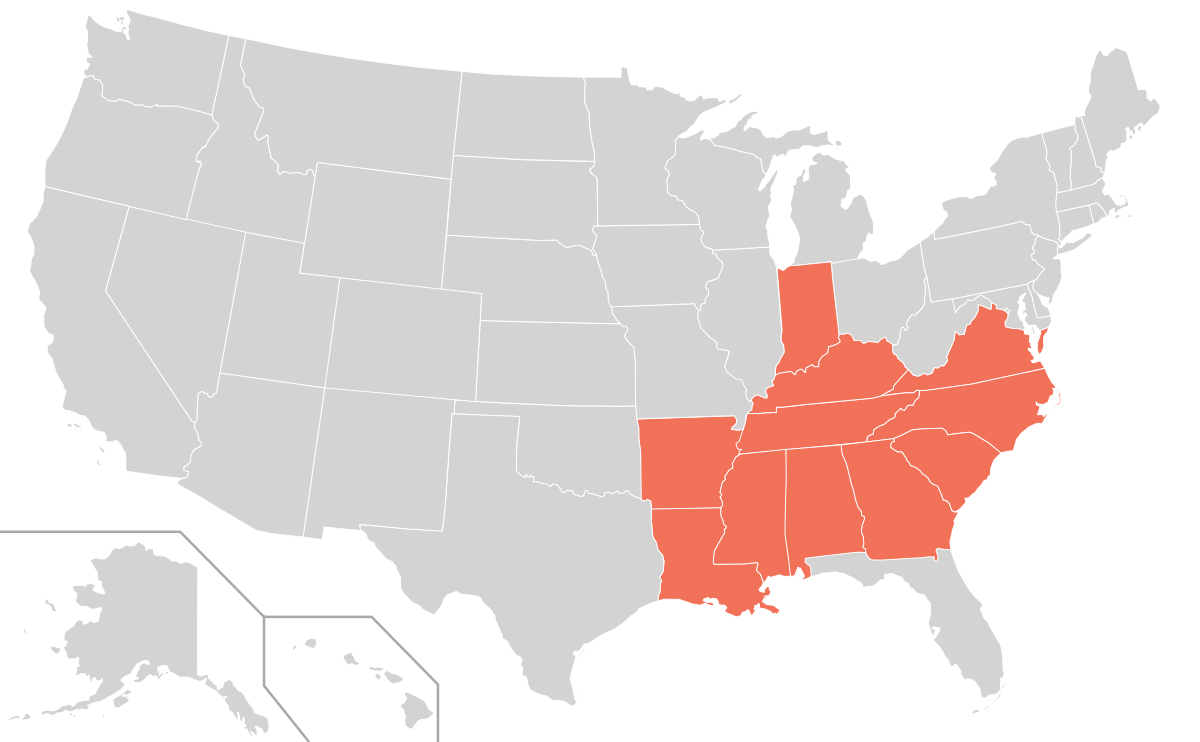
\includegraphics[width=0.9\textwidth,height=\textheight]{PresentationPhotos/strokeBelt.png}

}

\caption{States that are a part of the Stroke Belt, highlighted in
orange}

\end{figure}%
\end{frame}

\begin{frame}{Introduction}
\phantomsection\label{introduction-2}
\begin{itemize}
\item
  We chose to use the geographically weighted regression (GWR) model
  rather than other methods such as clustering and traditional linear
  regression for the following reasons:~

  \begin{itemize}
  \item
    The GWR model highlights the local spatial significance between the
    response variable and each covariate~
  \item
    We can analyze the spatial distribution, changes in percentage
    rates, and any correlations
  \end{itemize}
\end{itemize}
\end{frame}

\begin{frame}{Introduction}
\phantomsection\label{introduction-3}
\begin{itemize}
\tightlist
\item
  The concentrations of the covariates differ across the US so public
  health experts need to tailor to each region~
\item
  Because many factors influence CVD incidence rates, it's useful to use
  the GWR model to help health practitioners implement necessary
  intervention
\end{itemize}
\end{frame}

\section{Literature Review Section}\label{literature-review-section}

\begin{frame}{Literature Review}
\phantomsection\label{literature-review}
\begin{itemize}
\item
  For further context on our problem, we looked towards other research
  papers studying CVD using spatial analysis
\item
  Statistical regression + spatial models have been growing in
  popularity to analyze the distribution and factors of cardiovascular
  disease~
\item
  A good amount of other studies focus on socioeconomic covariates and
  their impact on cardiovascular disease mortality rates however, our
  study takes into account PM2.5 concentrations~
\item
  By analyzing the spatial distribution of our covariates, we can
  provide risk estimates for the year 2015
\end{itemize}
\end{frame}

\begin{frame}{Literature Review}
\phantomsection\label{literature-review-1}
\begin{itemize}
\item
  The geographically weighted model builds on the weighted least squares
  method and considers coefficients for each spatial unit for
  estimation~
\item
  We are interested in seeing the values that carry more weight because
  they carry a greater amount of influence
\end{itemize}
\end{frame}

\begin{frame}{Literature Review}
\phantomsection\label{literature-review-2}
\begin{itemize}
\item
  The ordinary least squares method generates global regression
  coefficients however it's prone to hidden spatial variability~
\item
  We use the GWR model to test and verify our results to be
  statistically significant, treating the OLS model as the null~
\item
  The GWR model minimizes errors between the actual and predicted
  values, which helps health practitioners narrow down the areas for
  improvement
\end{itemize}
\end{frame}

\section{Methods Section}\label{methods-section}

\begin{frame}{Methods}
\phantomsection\label{methods}
\begin{itemize}
\item
  Medicare claims, racial/geographic data were gathered from the Census
  and TIGER Bureau, median income was sourced from the Census API, air
  quality from NASA PM2.5 data, and unemployment rates were loaded from
  the Center for Disease Control (CDC).
\item
  The data was grouped by year, United States county, and coordinates
  for 2015; cleaned by removing entries with empty geometries and
  incomplete data, excluding Alaska and Hawaii, which led to Nantucket
  County being removed from the dataset
\end{itemize}
\end{frame}

\begin{frame}{Methods}
\phantomsection\label{methods-1}
\begin{itemize}
\item
  Transformed integrated data into a format suitable for Geographical
  Weighted Regression (GWR) by calculating centroids of the
  multi-polygon geometries to provide a single point to get precise
  location-based assessments.~
\item
  Cross-validation was utilized to estimate the optimal fixed bandwidth
  for the GWR model
\item
  The Gaussian kernel was chosen for its smoothness
\end{itemize}
\end{frame}

\begin{frame}{Model}
\phantomsection\label{model}
\(y = \beta_0*\%White +\beta_1* \%Black + \beta_2 *\%Hispanic + \beta_3 *\%Asian + \beta_4 *PM2.5 + \beta_5 * Median Income + \beta_6 * \%Unemployed\)

\begin{itemize}
\item
  A correction for the asymptotics of the t-values from the GWR model is
  required, as they do not follow a standard t-distribution

  \begin{itemize}
  \tightlist
  \item
    We adjusted the t-values of the GWR model, aligning the assessment
    of t-values with appropriate statistical significance testing.
  \end{itemize}
\end{itemize}
\end{frame}

\begin{frame}{Methods}
\phantomsection\label{methods-2}
\begin{itemize}
\item
  Geographic plots visualize the spatial distribution of CVD death rates
  across different US counties
\item
  Significance of various socioeconomic, environmental, and demographic
  factors on CVD death rates is analyzed regionally.
\end{itemize}
\end{frame}

\begin{frame}{Methods}
\phantomsection\label{methods-3}
\begin{figure}[H]

{\centering 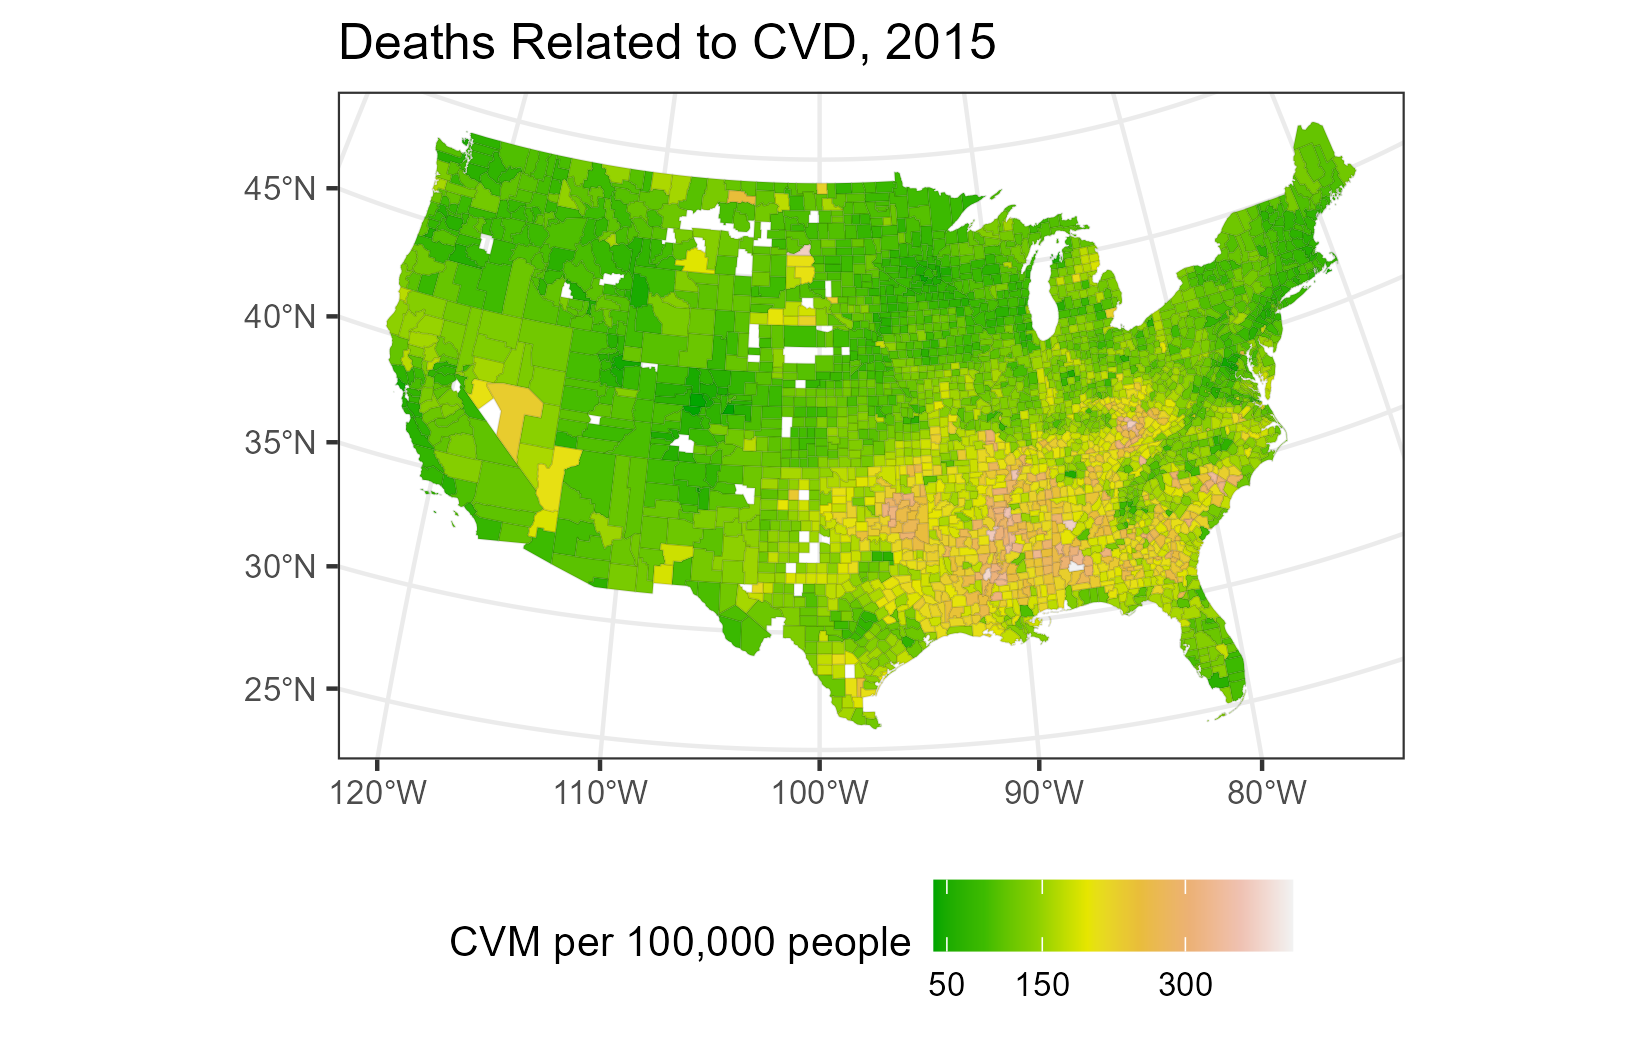
\includegraphics[width=0.8\textwidth,height=\textheight]{PresentationPhotos/edaplot.png}

}

\caption{Exploratory data analysis with full model. Many deaths are
shown to be concentrated in the Stroke Belt region.}

\end{figure}%
\end{frame}

\begin{frame}{Simulation}
\phantomsection\label{simulation}
\begin{figure}[H]

{\centering 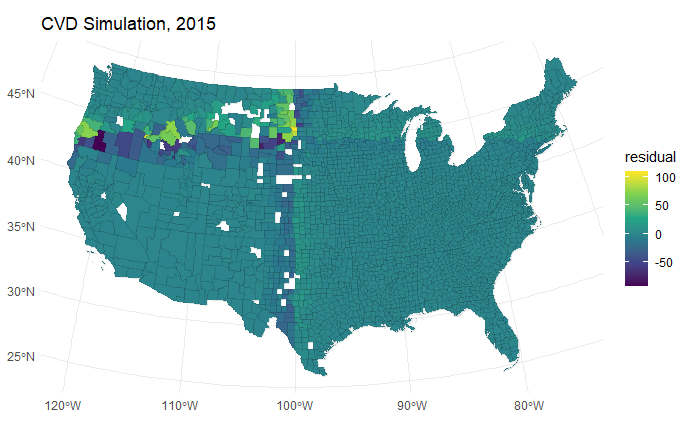
\includegraphics[width=0.8\textwidth,height=\textheight]{PresentationPhotos/simplot.png}

}

\caption{Simulated data is used with a piecewise function dividing the
geographical space into quadrants, each assigned different coefficients
to model spatial heterogeneity}

\end{figure}%
\end{frame}

\begin{frame}{Simulation}
\phantomsection\label{simulation-1}
\begin{longtable}[]{@{}lll@{}}
\caption{Moran's I, a spatial autocorrelation test, is performed on the
residuals of the GWR model. Results confirm a significant spatial
correlation.}\tabularnewline
\toprule\noalign{}
Moran I Statistic & Expectation & Variance \\
\midrule\noalign{}
\endfirsthead
\toprule\noalign{}
Moran I Statistic & Expectation & Variance \\
\midrule\noalign{}
\endhead
0.3010445156 & 0.0003274394 & 0.0001178233 \\
\bottomrule\noalign{}
\end{longtable}
\end{frame}

\section{Results Section}\label{results-section}

\begin{frame}{Results}
\phantomsection\label{results}
\begin{itemize}
\item
  The global regression model:

  \begin{itemize}
  \item
    Shows all predictors as statistically significant.
  \item
    Does not consider spatial correlation, potentially missing local
    variations.
  \item
    Residual analysis reveals spatial patterns, with clusters of higher
    and lower residuals indicating missed spatial variation.
  \end{itemize}
\end{itemize}

\begin{itemize}
\item
  The GWR model:

  \begin{itemize}
  \item
    Incorporates spatial variation, addressing a critical aspect of the
    data.
  \item
    Provides a more nuanced and realistic interpretation of how various
    factors affect death rates across different regions.
  \end{itemize}
\end{itemize}
\end{frame}

\begin{frame}{Results}
\phantomsection\label{results-1}
\begin{figure}[H]

{\centering 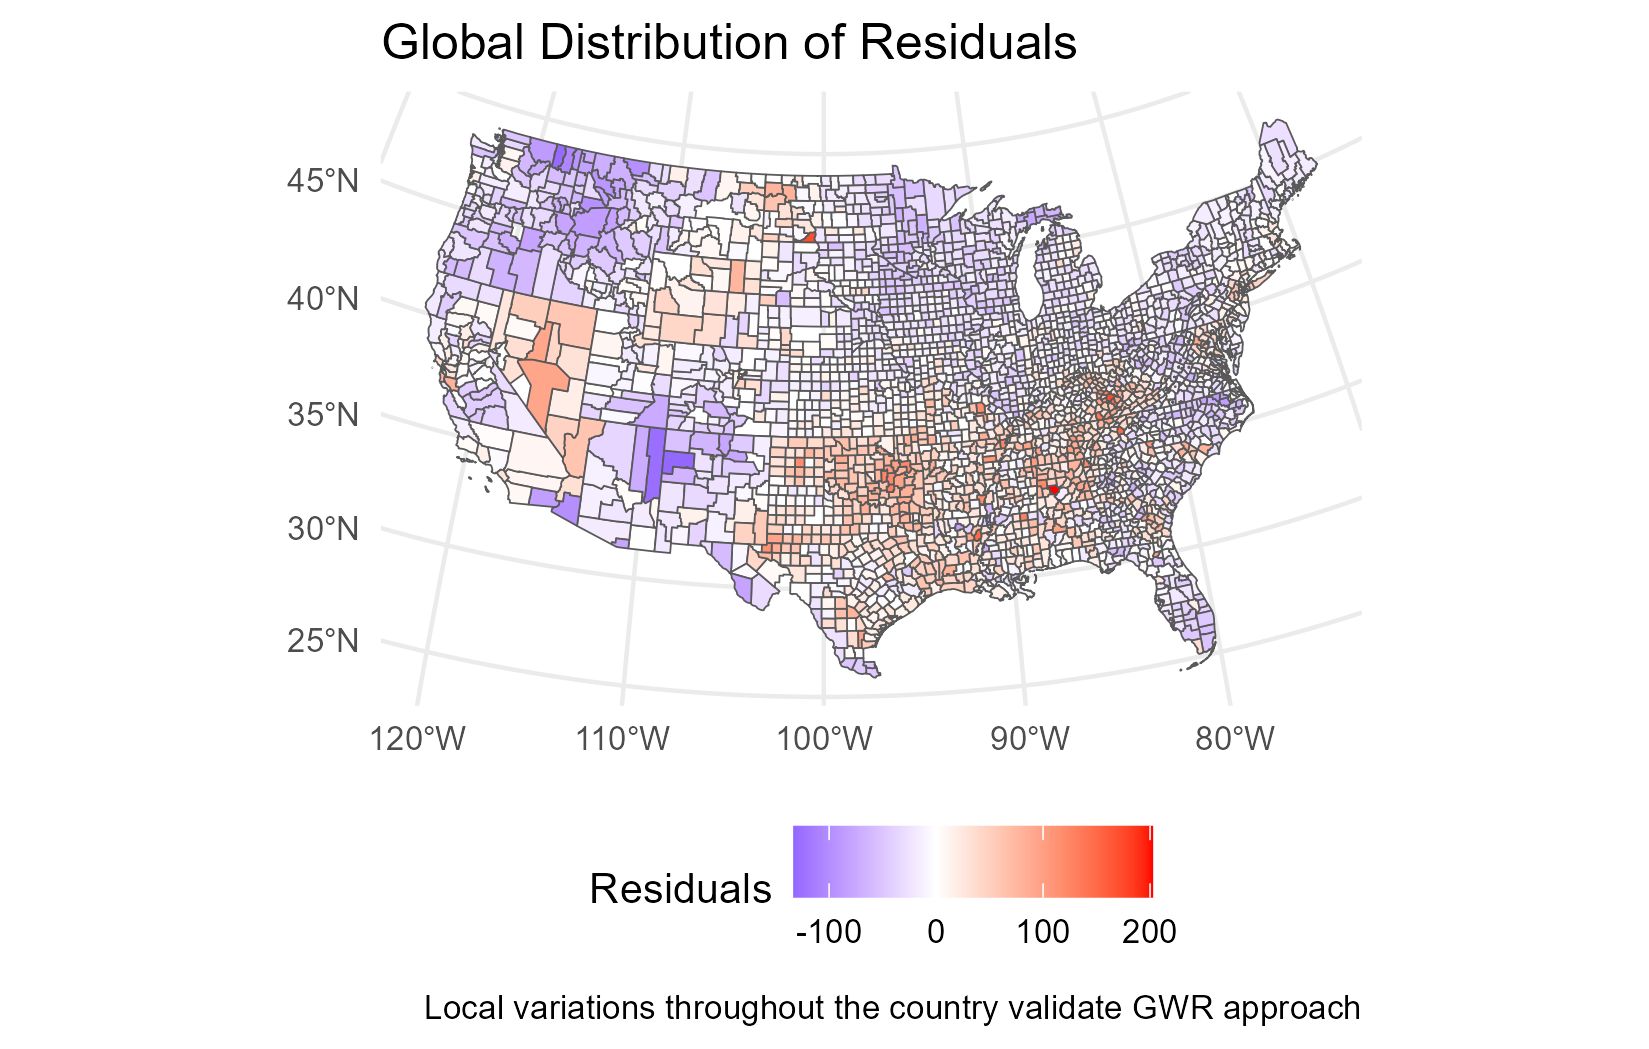
\includegraphics{PresentationPhotos/gdrplot.png}

}

\caption{Local variations are critical for understanding the nature of
our data}

\end{figure}%
\end{frame}

\begin{frame}{Results}
\phantomsection\label{results-2}
\begin{figure}[H]

{\centering 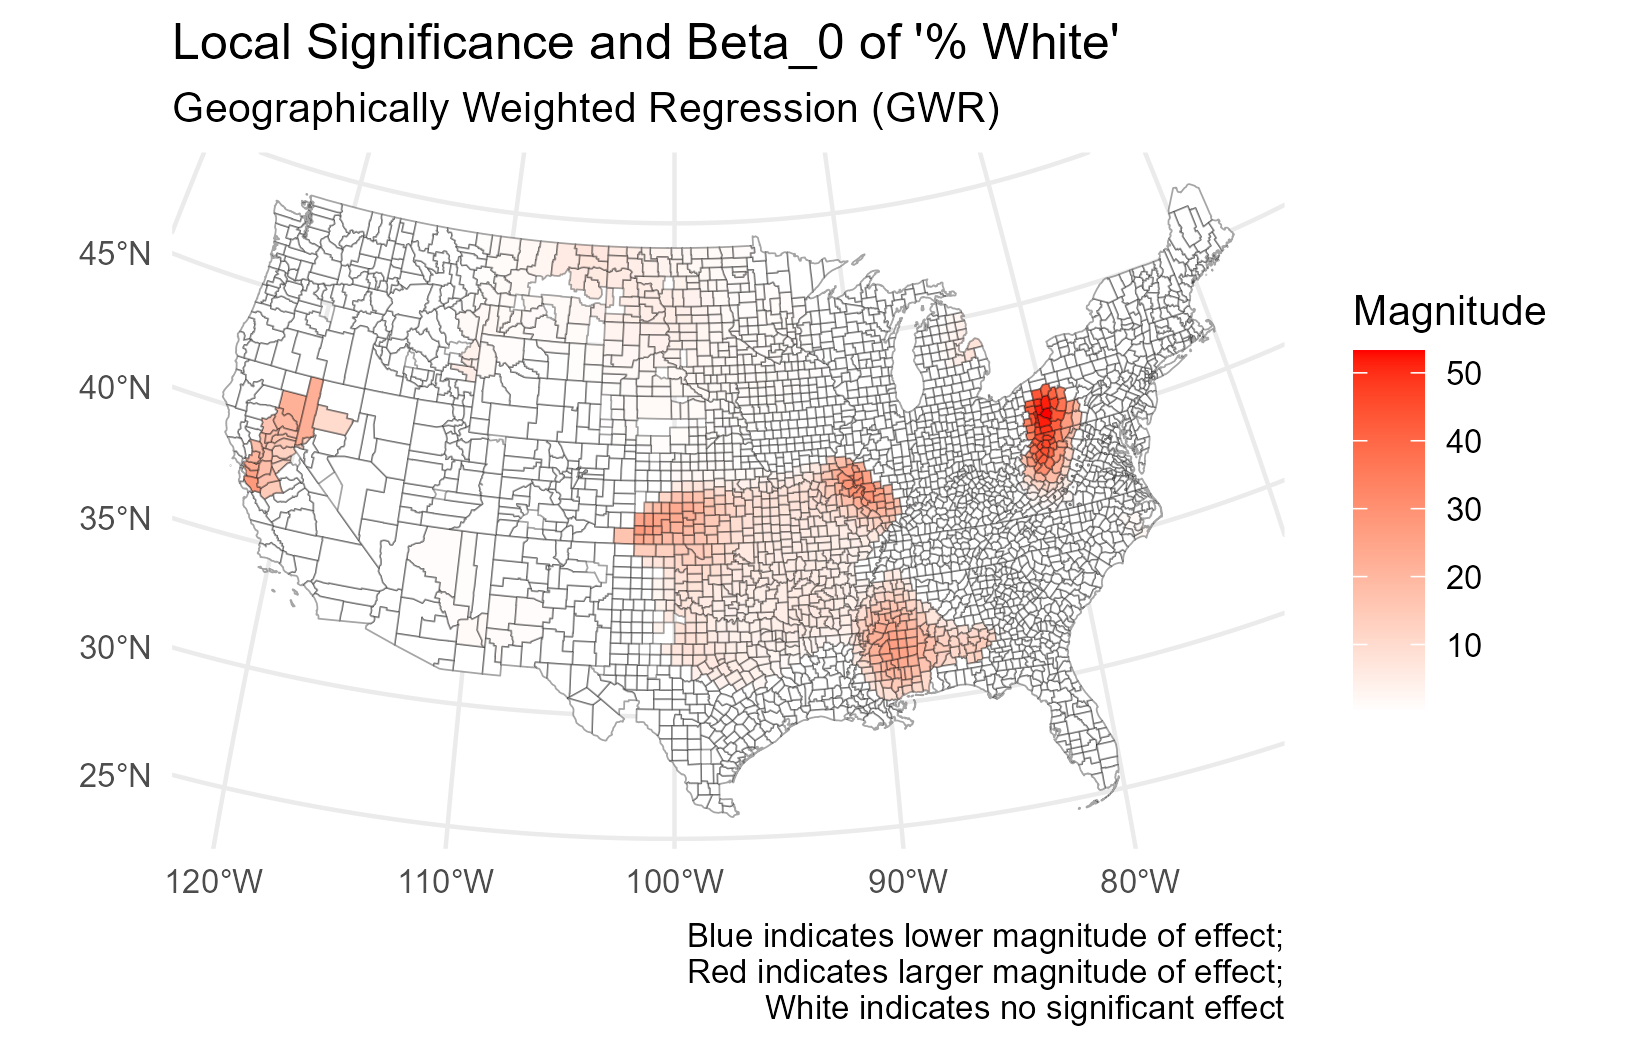
\includegraphics[width=0.9\textwidth,height=\textheight]{PresentationPhotos/whiteplot.png}

}

\caption{Significant negative correlation in central and southeastern
regions. Positive correlation near New Mexico and Arizona.}

\end{figure}%
\end{frame}

\begin{frame}{Results}
\phantomsection\label{results-3}
\begin{figure}[H]

{\centering 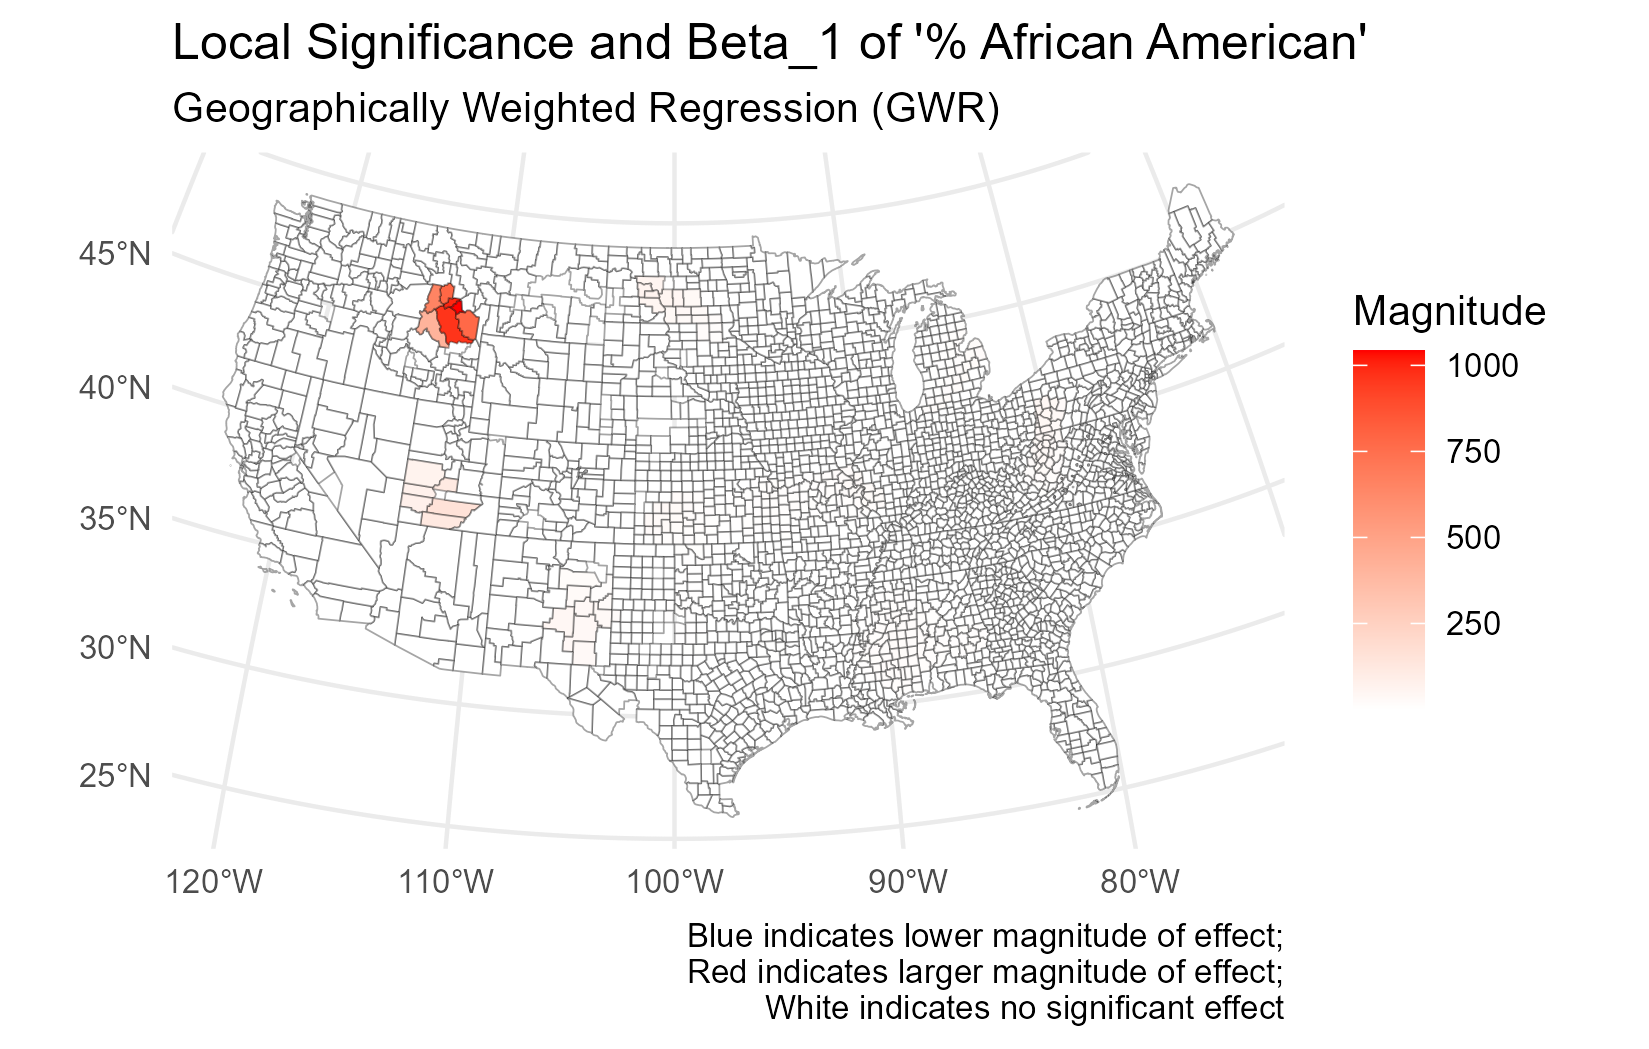
\includegraphics[width=0.9\textwidth,height=\textheight]{PresentationPhotos/blackplot.png}

}

\caption{Significant positive correlation in northern central region.
Significant negative correlation in central to southeastern areas.}

\end{figure}%
\end{frame}

\begin{frame}{Results}
\phantomsection\label{results-4}
\begin{figure}[H]

{\centering 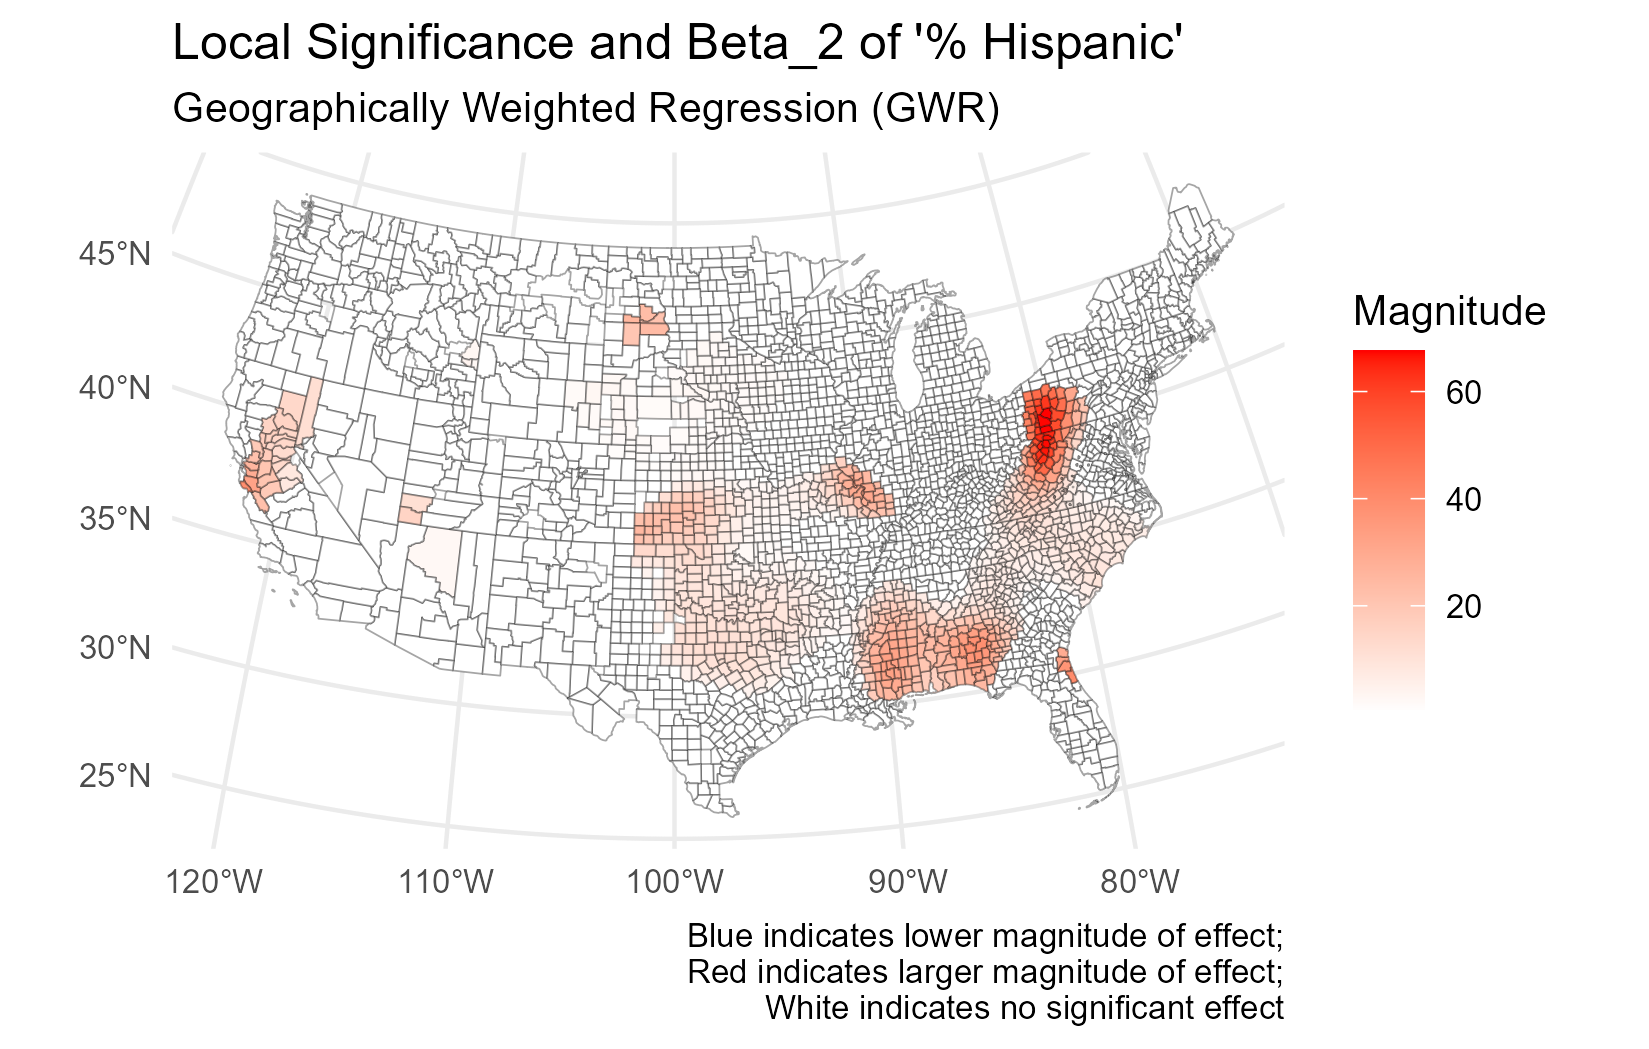
\includegraphics[width=0.9\textwidth,height=\textheight]{PresentationPhotos/hispanplot.png}

}

\caption{Significant negative correlation across central and
southeastern regions. Isolated red patches in north-central suggest
positive correlations.}

\end{figure}%
\end{frame}

\begin{frame}{Results}
\phantomsection\label{results-5}
\begin{figure}[H]

{\centering 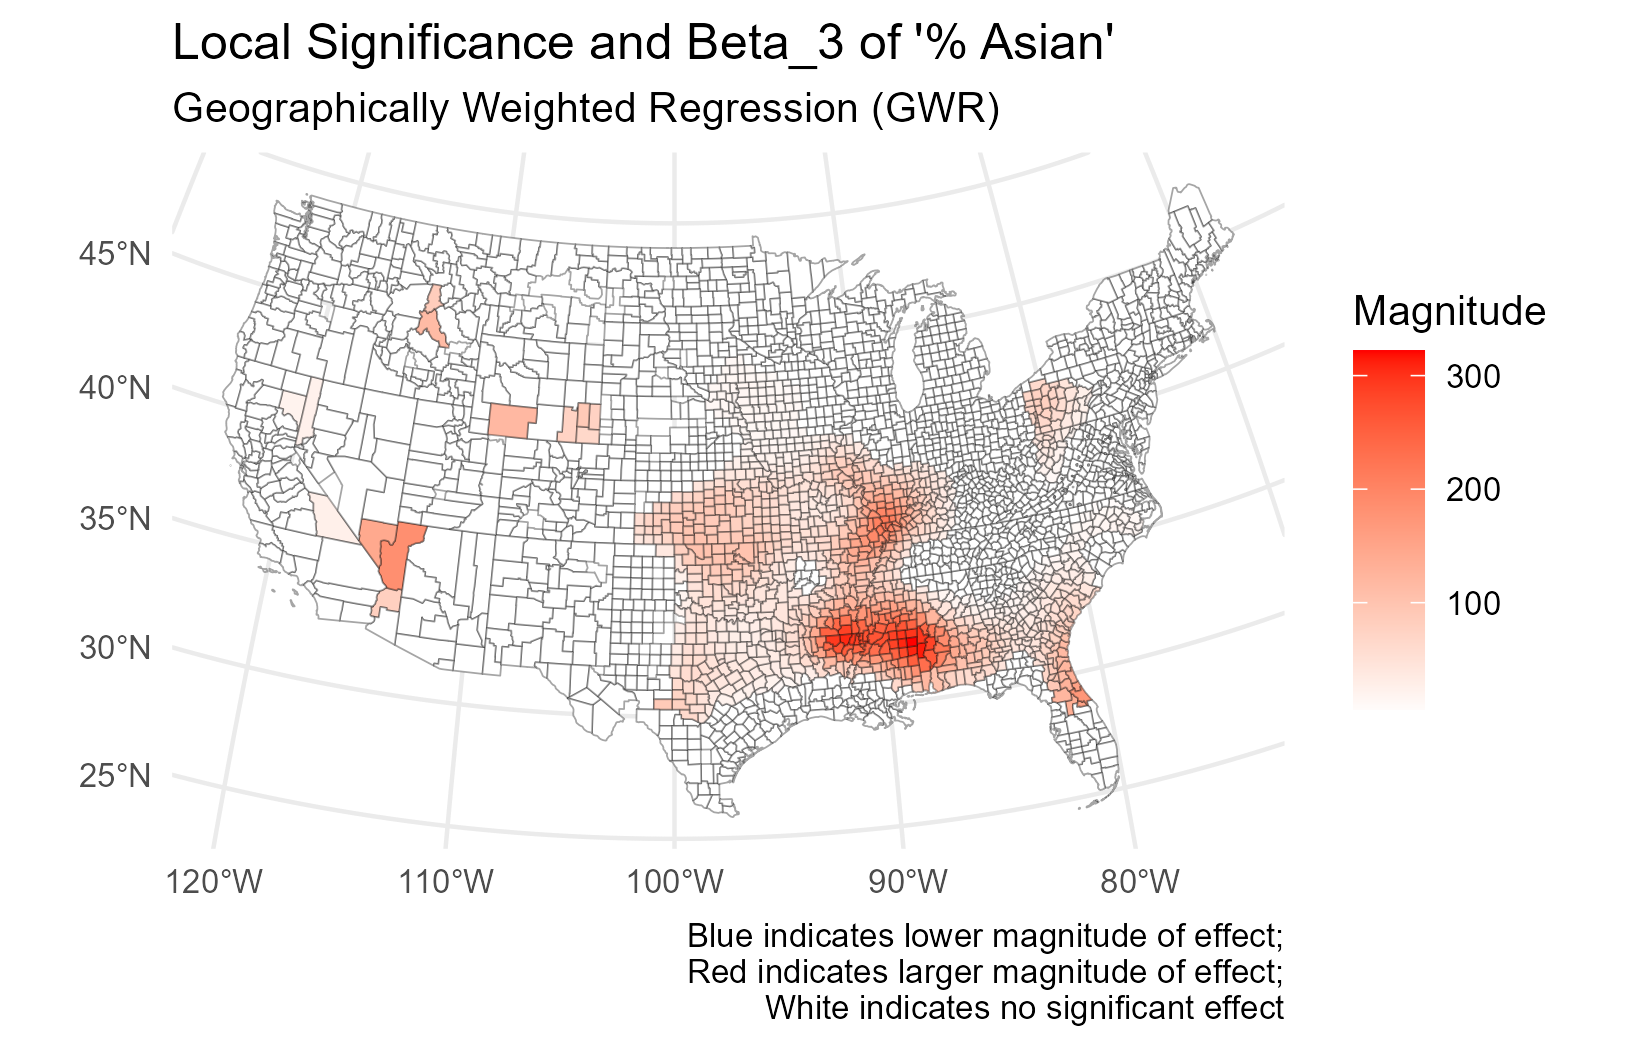
\includegraphics[width=0.9\textwidth,height=\textheight]{PresentationPhotos/asianplot.png}

}

\caption{Generally, increased \% Asian correlates with lower CVD
outcomes in central to eastern regions. Some western regions show
positive correlations.}

\end{figure}%
\end{frame}

\begin{frame}{Results}
\phantomsection\label{results-6}
\begin{figure}[H]

{\centering 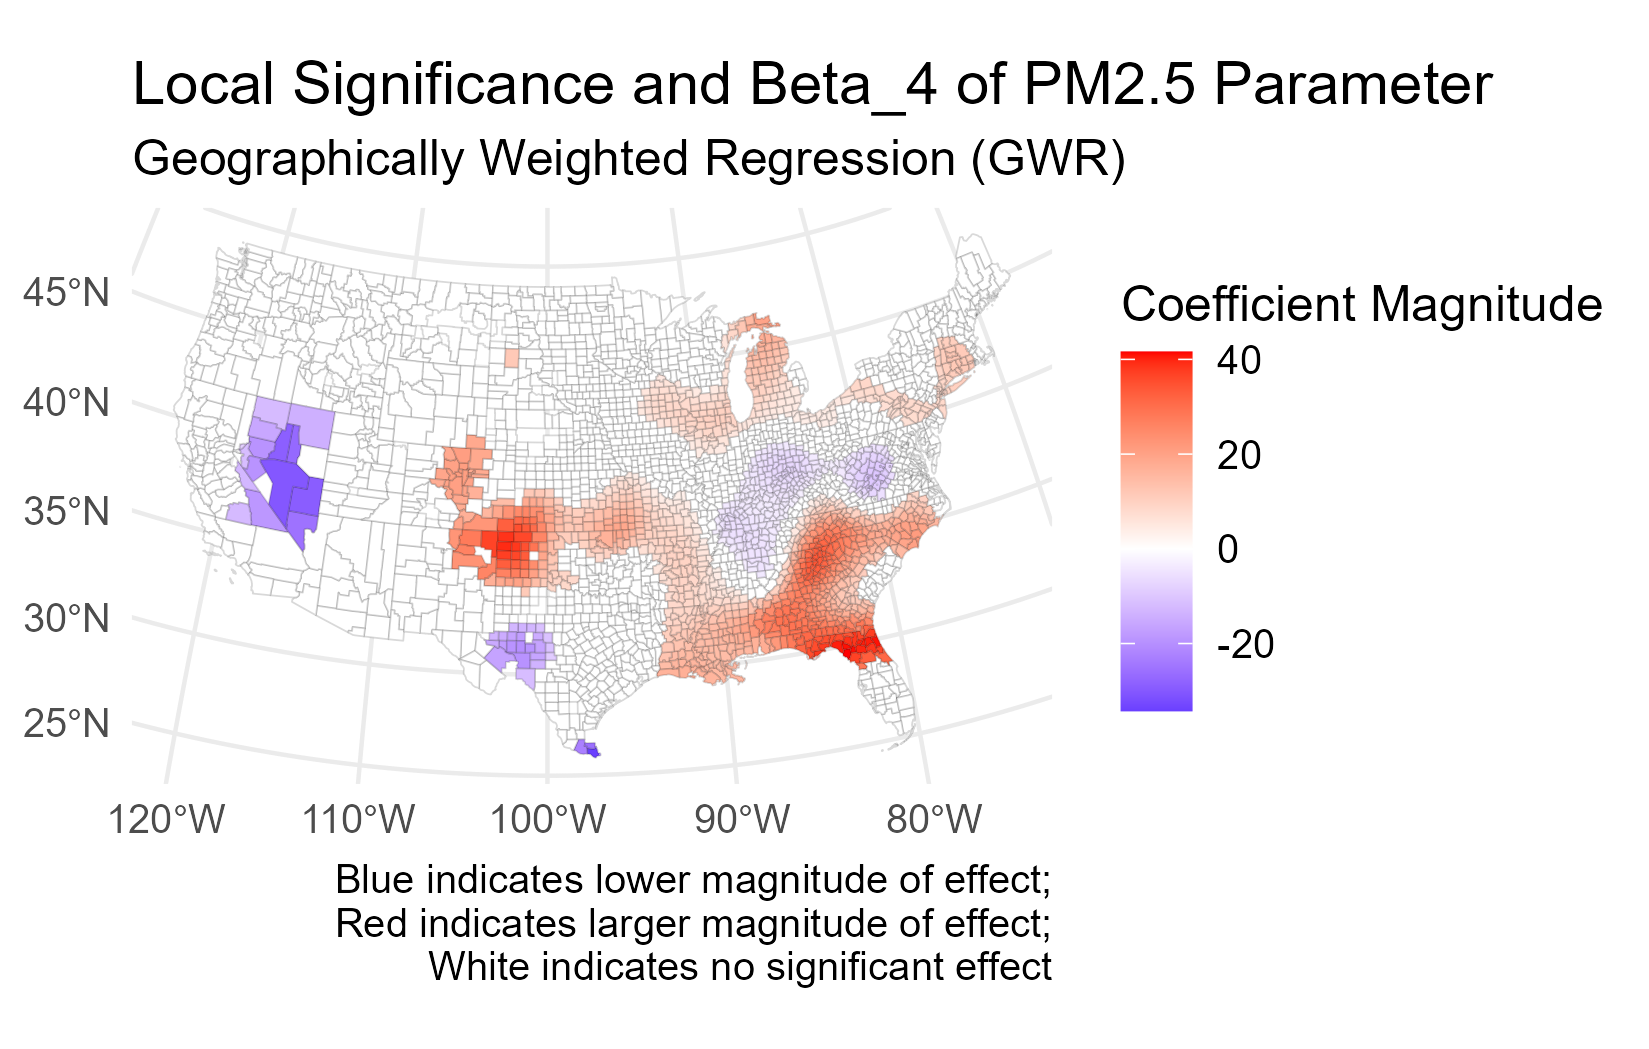
\includegraphics[width=0.9\textwidth,height=\textheight]{PresentationPhotos/pm25.png}

}

\caption{Higher levels in southern and northeastern regions correlate
with higher CVD rates. Negative correlations in some western regions.}

\end{figure}%
\end{frame}

\begin{frame}{Results}
\phantomsection\label{results-7}
\begin{figure}[H]

{\centering 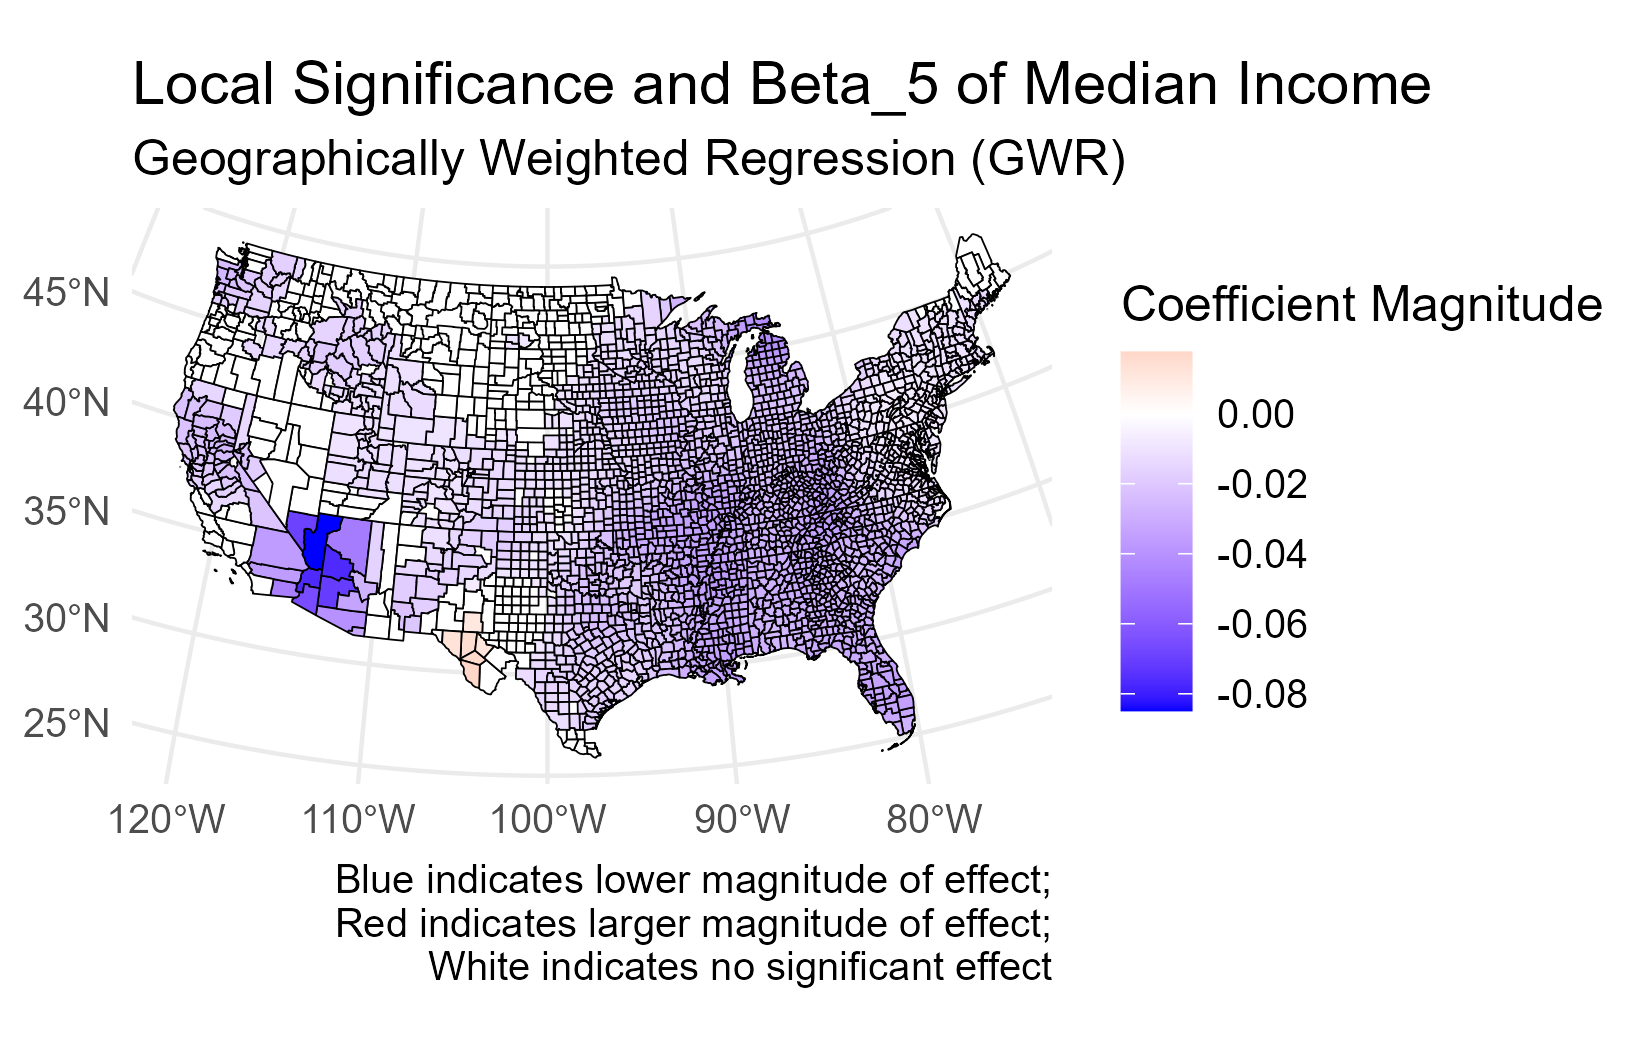
\includegraphics[width=0.9\textwidth,height=\textheight]{PresentationPhotos/medIncomePlot.png}

}

\caption{Generally, higher median income correlates with lower CVD
outcomes. Notable exception in parts of Texas with a positive
correlation.}

\end{figure}%
\end{frame}

\begin{frame}{Results}
\phantomsection\label{results-8}
\begin{figure}[H]

{\centering 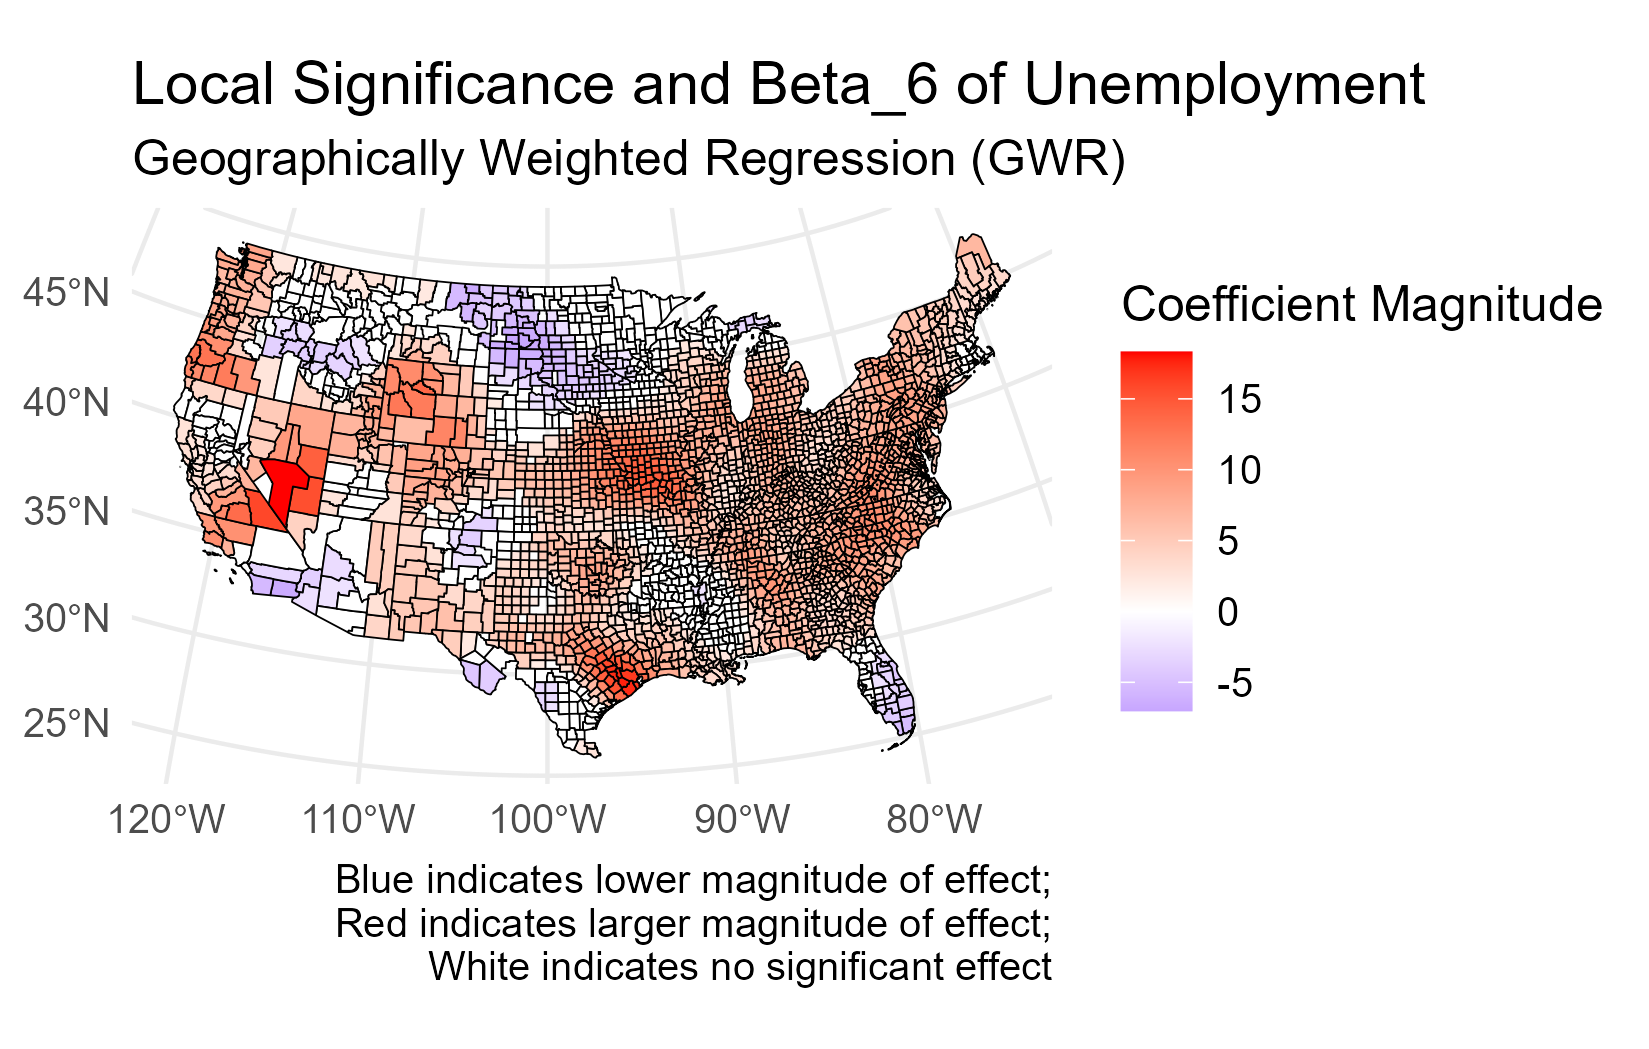
\includegraphics[width=0.9\textwidth,height=\textheight]{PresentationPhotos/unemployPlot.png}

}

\caption{Mostly positive correlation with CVD rates in central regions.
Negative correlation in southwestern regions.}

\end{figure}%
\end{frame}

\section{Discussion Section}\label{discussion-section}

\begin{frame}{Discussion}
\phantomsection\label{discussion}
\begin{itemize}
\tightlist
\item
  The purpose of the study was to fill a gap in CVD research that
  primarily focused on the stroke belt and adults over 55, with the goal
  of answering: what are the socioeconomic and environmental factors
  affecting CVD rates in the U.S.?
\end{itemize}

\begin{figure}[H]

{\centering 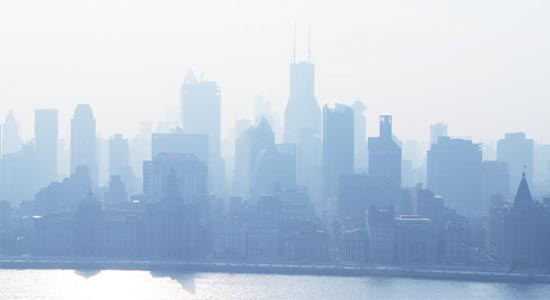
\includegraphics[width=0.75\textwidth,height=\textheight]{PresentationPhotos/urbanPollution.jpg}

}

\caption{Urban smog in Chinese city}

\end{figure}%
\end{frame}

\begin{frame}{Discussion}
\phantomsection\label{discussion-1}
\begin{itemize}
\item
  The prior maps showed that factors are highly localized for most of
  our covariates
\item
  Expected exception for median income, which has a constant effect
  regardless of region
\end{itemize}
\end{frame}

\begin{frame}{Discussion}
\phantomsection\label{discussion-2}
\begin{itemize}
\item
  We observed localized impacts for African Americans, Hispanics, and
  Asians in different areas of the country
\item
  Limitation in race percentages presented by misreporting of medical
  records affecting minorities (Tabb et al.~2020). Shows that
  intervention is needed to combat racial health disparities that were
  caused by disparities in the healthcare system.
\end{itemize}
\end{frame}

\begin{frame}{Variance Inflation Factor (VIF)}
\phantomsection\label{variance-inflation-factor-vif}
\begin{itemize}
\item
  Looking at the Variance Inflation Factor (VIF) of our GWR model:

  \begin{tabular}{rrrrrrr}
    \hline
  \%WT & \%BLK & \%HISP & \%AS & PM2.5 & Income & Unemp. \\ 
    \hline
  183.00 & 196.00 & 7.00 & 3.00 & 1.00 & 2.00 & 3.00 \\ 
    81.00 & 94.00 & 4.00 & 3.00 & 2.00 & 3.00 & 3.00 \\ 
    302.00 & 314.00 & 17.00 & 4.00 & 1.00 & 2.00 & 2.00 \\ 
    141.00 & 151.00 & 5.00 & 2.00 & 1.00 & 2.00 & 3.00 \\ 
    132.00 & 128.00 & 8.00 & 3.00 & 1.00 & 2.00 & 2.00 \\ 
    283.00 & 294.00 & 14.00 & 4.00 & 1.00 & 2.00 & 2.00 \\ 
     \hline
  \end{tabular}
\end{itemize}

We can see that the \%WT and \%BLK columns have disproportionately high
values. This represents a limitation in the model as it suggests
multicollinearity.
\end{frame}

\begin{frame}{Variance Inflation Factor}
\phantomsection\label{variance-inflation-factor}
This is, however, to be expected given that the racial variables we are
using sum up to one. An adjustment to the model could be made in a
future study to eliminate the \% White variable and aggregate the other
three races into a single \% Non-White variable.
\end{frame}

\begin{frame}{Discussion}
\phantomsection\label{discussion-3}
\begin{itemize}
\tightlist
\item
  PM2.5 concentrations in the central and southeastern regions of the
  United States suggest that region-specific intervention may be needed.
\end{itemize}

\begin{figure}[H]

{\centering 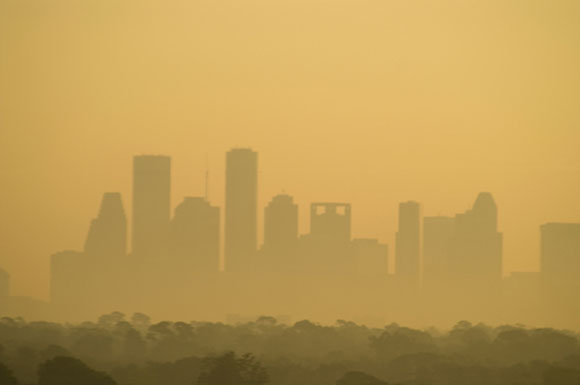
\includegraphics[width=0.75\textwidth,height=\textheight]{PresentationPhotos/Houston-Smog.jpg}

}

\caption{Particulate smog in Houston, Texas}

\end{figure}%
\end{frame}

\section{Conclusion}\label{conclusion}

\begin{frame}{Conclusion}
\phantomsection\label{conclusion-1}
\begin{itemize}
\item
  We have shown that a GWR model can be used to analyze the relationship
  between CVM and socioeconomic covariates.
\item
  The differing local significance that we detected highlights the need
  to identify region-specific interventions to curb the toll of CVD.
\end{itemize}
\end{frame}



\end{document}
